\capitulo{SISTEMA DESENVOLVIDO}

\iniciocapitulo
Todo início de semestre instituições de ensino se deparam com o PAS, um problema de alocação de salas que tem sua complexidade definia como NP-Difícil. Logo a resolução manual de problemas desse tipo se torna inviável em um espaço de tempo curto. Para isto são utilizadas meta-heurísticas que são métodos de aproximação, que ajudam a encontrar uma solução em um conjunto de soluções viáveis. Este trabalho utiliza informações fornecidas pela FAFICH UFMG, nestas informações estão contidas salas com suas propriedades, e disciplinas enviadas pelos colegiados com suas restrições de horários e informações básicas de cada uma. A resolução do problema PAS consiste então na alocação de todas as disciplinas enviadas pelos colegiados respeitando as restrições do problema. A técnica utilizada para tentar solucionar o problema é chamada de algoritmo genético uma meta-heurística bastante utilizada na resolução de problemas deste tipo.\par

\secao{Modelagem}

\subsecao{Diagramas de caso de uso}

A Figura~\ref{fig:casodeuso} descreve todas as funcionalidades que o sistema possui. Essas funcionalidades foram dividias em 2 atores, "Gerente" e "Sistema", cada um ligado com suas respectivas funcionalidades, porém, o "Gerente" pode acessar o ator "Sistema" para ter acessos funcionalidades que são encontradas no mesmo. O sentido das setas informa o que cada ator pode acessar no sistema.\par

\begin{figure}[!htb]
\caption[Diagrama de Caso de Uso]{Diagrama de Caso de Uso}
\label{fig:casodeuso}
\centering
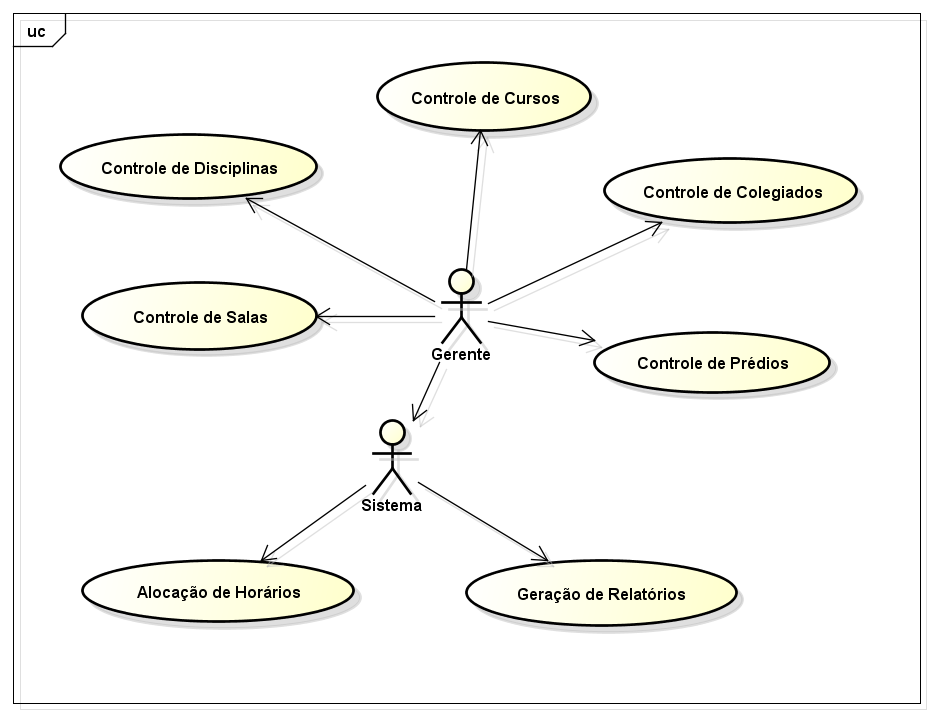
\includegraphics[scale=0.5]{imagens/diagramaCasoUso.png}
\\ \textbf{\footnotesize Fonte: Desenvolvido pelo autor}
\end{figure}

As funcionalidades "controle de turnos", "controle de horários", "controle de prédios", "controle de salas", "controle de cursos", "controle de colegiados", "controle de períodos" e "controle de disciplinas" são disponibilizadas através de módulos com as funcionalidades \textit{Create, Read, Update, Delete} (CRUD) para que o responsável tenha total controle sobre as informações a serem administradas.\par

Já as funcionalidades "alocação de horários" e "geração de relatórios", são rotinas executadas pelo "Sistema". A funcionalidade alocação de horários é uma rotina que utiliza conceitos de algoritmo genético para encontrar a melhor solução do problema e a funcionalidade geração de relatórios mostra para o "Gerente" o melhor resultado de alocação encontrado pelo algoritmo. Detalhes do funcionamento serão explicados nas seções posteriores.\par

\subsecao{Diagrama de Entidade Relacionamento}

A Figura~\ref{fig:der} mostra o relacionamento das tabelas no sistema atraves do diagrama de entidade relacionamento.\par

\begin{figure}[!htb]
\caption[Diagrama de Entidade Relacionamento]{Diagrama de Entidade Relacionamento}
\label{fig:der}
\centering
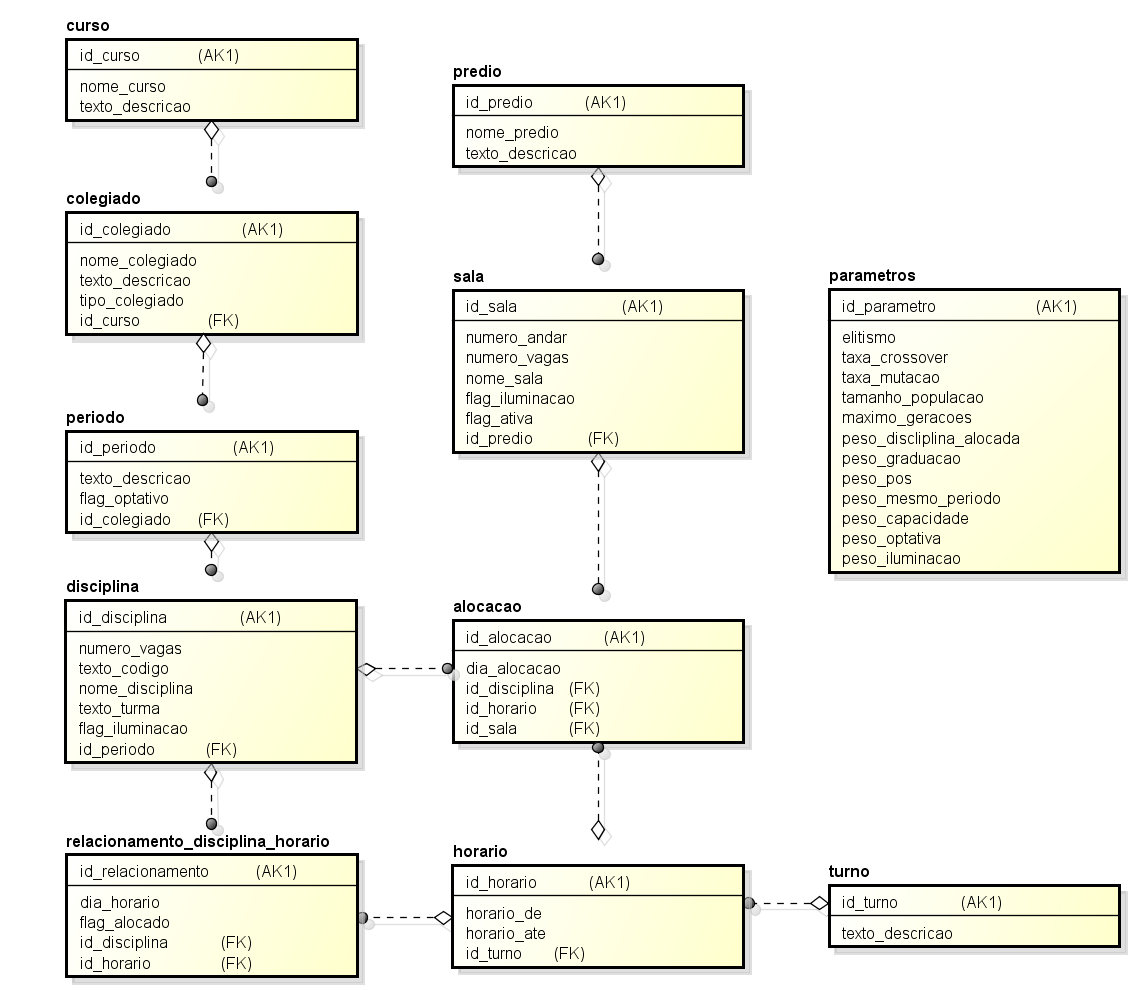
\includegraphics[scale=0.5]{imagens/diagramaEntidadeRelacionamento.png}
\\ \textbf{\footnotesize Fonte: Desenvolvido pelo autor}
\end{figure}

As tabelas curso, colegiado, período, disciplina, sala, prédio, turno, horário são utilizadas para armazenar as informações dos respectivos objetos que são controlados pelos módulos de CRUD e suas respectivas funcionalidades.\par

A tabela relacionamento\_disciplina\_horário, salva as obrigatoriedades dos horários das disciplinas, uma vez que, todos os horários são montados pelos colegiados e não pelo responsável pela alocação das disciplinas nas salas.\par

A tabela alocação contem o relacionamento de disciplina, horário e sala o que corresponde a melhor alocação encontrada pelo algoritmo. O item disciplina pode ter o seu valor como nulo o que significa que em um especifico horário e em uma determinada sala não existe disciplina alocada.\par

A tabela parâmetro é utilizada apenas para guardar os últimos parâmetros utilizados na execução do algoritmo genético.\par


\subsecao{Diagramas de classe}

Este diagrama é das classes do algoritmo genético, as classes do sistema em geral não serão abordados. Quando terminar o codigo revisar e explicar.\par
~\ref{fig:dc}
\begin{figure}[!htb]
\caption[Diagrama de Classe]{Diagrama de Classe}
\label{fig:dc}
\centering
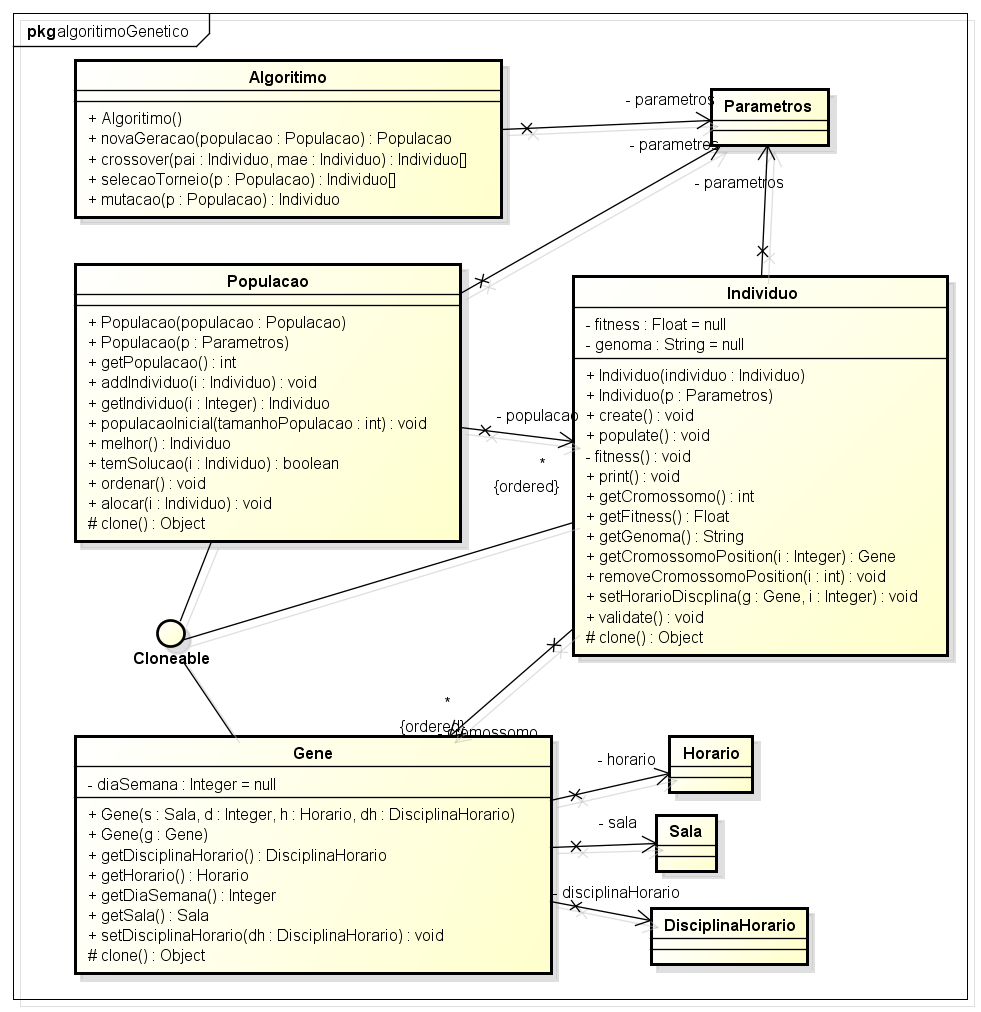
\includegraphics[scale=0.5]{imagens/diagramaClasse.png}
\\ \textbf{\footnotesize Fonte: Desenvolvido pelo autor}
\end{figure}

\secao{algoritmo Genético}

Após a da modelagem do sistema com pleno conhecimento do problema e o levantamento bibliográfico sobre algoritmos genéticos, foi feito o relacionamento do problema com os termos da biologia.\par

\subsecao{Indivíduo}

O termo gene representado pela figura~\ref{fig:gene} possui uma combinação de quatro variáveis sala, dia da semana, horário e o relacionamento de obrigatoriedade 
"disciplina horário". As variáveis sala, horário e dia da semana são fixas, não podem ser nulas uma vez que todas as combinações possíveis destas três variáveis formam um cromossomo que tem um tamanho fixo para todos os indivíduos. \par

Um gene com o relacionamento "disciplina horário" igual a nulo representa um horário vago para aquela combinação especifica de sala, horário e dia da semana.\par

\begin{figure}[!htb]
\caption[Representação Gene]{Representação Gene}
\label{fig:gene}
\centering
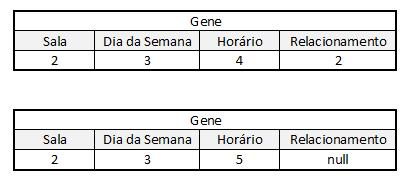
\includegraphics[scale=0.7]{imagens/representacaoGene.png}
\\ \textbf{\footnotesize Fonte: Desenvolvido pelo autor}
\end{figure}

Um cromossomo é uma sequência de genes, esta sequência tem um tamanho fixo e pode ser medido pela seguinte fórmula.

$$(número de Salas * número de Horários * número de dias da semana)$$

Inicialmente o individuo contem todas as variáveis relacionamentos de obrigatoriedade nulas, estas variáveis serão preenchidas randomicamente na criação da população inicial que em breve será explicada. O cromossomo do indivíduo preenchido com os relacionamentos de obrigatoriedades representa uma alocação. Está alocação é medida pela sua pontuação de \textit{fitness} que será apresentado  em outro tópico, podendo ser ou não o resultado do problema. Os valores utilizados na representação do cromossomo. A figura~\ref{fig:cromossomo} são os ID's do relacionamento de obrigatoriedade entre horário e disciplina. Em caso de horário vago em um determinado gene esta variável terá o valor nulo.\par

\begin{figure}[!htb]
\caption[Representação Cromossomo]{Representação Cromossomo}
\label{fig:cromossomo}
\centering
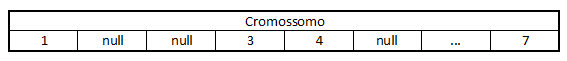
\includegraphics[scale=0.8]{imagens/representacaoCromossomo.png}
\\ \textbf{\footnotesize Fonte: Desenvolvido pelo autor}
\end{figure}

O termo indivíduo é então composto pelo cromossomo juntamente com a pontuação adquirida após a execução do método calculo de \textit{fitness}, a figura~\ref{fig:individuo} demonstra a representação de um indivíduo.\par

\begin{figure}[!htb]
\caption[Representação Individuo]{Representação Individuo}
\label{fig:individuo}
\centering
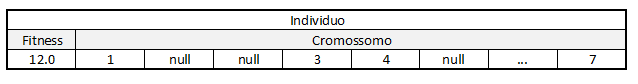
\includegraphics[scale=0.8]{imagens/representacaoIndividuo.png}
\\ \textbf{\footnotesize Fonte: Desenvolvido pelo autor}
\end{figure}

\subsecao{Definição da função objetivo}

O calculo da função objetivo é realizado através da execução da fórmula apresentada a seguir para calcular cada restrição. O calculo da primeira restrição chamada de \textit{fitness01} que se trata da restrição de obrigatoriedade entre as disciplinas e horários, é realizado um somatório de todos relacionamentos de obrigatoriedade que estão em uma posição correta acordo com os dados contidos no gene em que está alocado em seguida, utilizando o somatório dos relacionamento que estão em sua posição correta é aplicada a regra de 3.


$$fitness01 = \sum_{i=1}^n * 100 / contDisciplinaHorario$$ 

O mesmo calculo é realizado para as outras restrições, utilizando o somatório das disciplinas que tem os horários estão na mesma sala chamamos de \textit{fitness02}, e disciplinas que a capacidade da sala é atendida \textit{fitness03}.

O fitness final é calculado pela formula este calculo tem como valor máximo 100 e minimo 0.

$$ (fitness01+fitness02+fitness03)/3 $$ 



\subsecao{Operadores genéticos}

Um dos operadores genéticos utilizados neste trabalho conforme citado anteriormente é o elitismo. Este operador genético com valor verdadeiro garante a seleção 20\% dos melhores indivíduos para a próxima geração.\par

Mutação é a inversão genética dos genes de um indivíduo, escolhido randomicamente, da população anterior. Apos a realização da mutação genética o individuo é inserido na nova população.\par

Primeiramente são escolhidos de forma randômica dois genes do cromossomo. Apos a escolha dos genes a serem trocados, é feita a troca dos genes de posição. No caso apenas a relação de obrigatoriedade é trocada, permanecendo as outras propriedades, então retornado um novo indivíduo que tem a composição genética alterada. Apos a mutação este indivíduo recebe uma nova nota de \textit{fitness} de acordo com a sua nova sequencia de genes. Está nota pode ser maior ou menor do que a anterior a figura ~\ref{fig:mutacao} representa o processo descrito.\par

\begin{figure}[!htb]
\caption[Representação Mutação]{Representação Mutação}
\label{fig:mutacao}
\centering
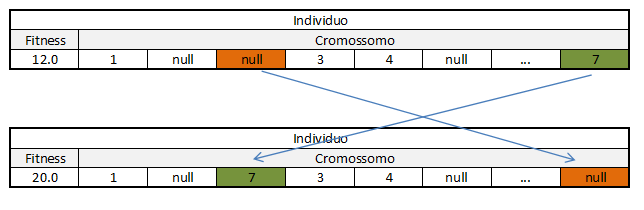
\includegraphics[scale=0.7]{imagens/representacaoMutacao.png}
\\ \textbf{\footnotesize Fonte: Desenvolvido pelo autor}
\end{figure}

O método seleção por torneio é utilizado para selecionar os indivíduos que iram participar do \textit{crossover}. O método escolhe três indivíduos da população anterior randomicamente e dos três indivíduos escolhidos, os dois que contêm a maior pontuação de \textit{fitness} são selecionados e enviados para o \textit{crossover}.\par

Para o método de \textit{crossover} inicialmente é escolhido um ponto de corte para se realizar o cruzamento entres os pais (pai e mãe). A figura~\ref{fig:antesCross} apresenta os indivíduos antes do cruzamento e o indivíduo pai marcado com o ponto de corte.\par

\begin{figure}[!htb]
\caption[Indivíduos antes do crossover]{Indivíduos antes do crossover}
\label{fig:antesCross}
\centering
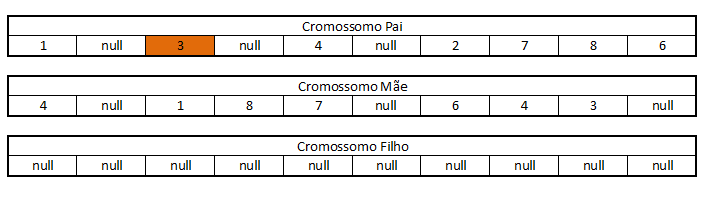
\includegraphics[scale=0.7]{imagens/individuosAntesInsersaoGenetica.png}
\\ \textbf{\footnotesize Fonte: Desenvolvido pelo autor}
\end{figure}

Após a escolha o filho 1 recebe todos os genes contidos no pai que estão antes do valor do ponto de corte. Devemos lembrar que o filho é um indivíduo e que os mesmo já contem o numero de genes pré definidos e nulos quando criados. Quando ocorre a troca genética estamos falando do envio das obrigatoriedades das disciplinas em relação aos horários. Para que não ocorra a repetição das informações contidas no pai e na mãe, os genes já utilizados no ponto de corte são removidos do indivíduo mãe. A marca no cromossomo filho representa o ponto de corte. Conforme apresentado na figura~\ref{fig:materialPai}.

\begin{figure}[!htb]
\caption[Inserção do material genético do pai]{Inserção do material genético do pai}
\label{fig:materialPai}
\centering
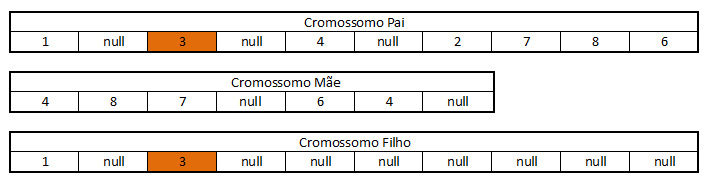
\includegraphics[scale=0.6]{imagens/individuosAposInsersaoGenetica.png}
\\ \textbf{\footnotesize Fonte: Desenvolvido pelo autor}
\end{figure}

Ao término da adição dos genes do ponto de corte o filho 1 recebe as informações genéticas que faltavam da mãe. A figura~\ref{fig:materialMae} representa como os indivíduos ficaram após a operação.

\begin{figure}[!htb]
\caption[Inserção do material genético da mãe]{Inserção do material genético da mãe}
\label{fig:materialMae}
\centering
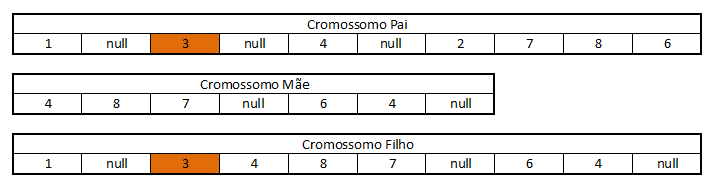
\includegraphics[scale=0.7]{imagens/insersaoMaterialMae.png}
\\ \textbf{\footnotesize Fonte: Desenvolvido pelo autor}
\end{figure}

Este mesmo processo é realizado para a criação do filho 2, porém, ao criar este novo filho, devemos trocas as operações realizadas entre o pai e a mãe invertendo os mesmo de lugar no fluxo descrito.

Após a realização do \textit{crossover} os filhos recebem uma nova nota de \textit{fitness} que conforme dito anteriormente podendo ser maior ou menor do que a anterior.
\subsecao{População}

Uma população, quando relacionada aos termos genéticos, se trata de um conjunto de indivíduos, também representa uma interação do algoritmo genético, ou seja uma geração. A manipulação da população e de suas propriedades é feita através de parâmetros, enviados antes da execução do algoritmo. Estes parâmetros são elitismo, taxa de \textit{crossover}, taxa de mutação, tamanho da população e número máximo de gerações.

De acordo com os parâmetros passados é criada a população inicial. Para cada indivíduo criado é utilizado um método para inserir randomicamente todos os registros de relacionamento de obrigatoriedade entre disciplina e horário em cada um dos genes que previamente foram criados como nulos, estes indivíduos são criados até que a população atinga o tamanho da população que deve ser igual ao parâmetro tamanho da população.\par

Para cada geração, é criada uma nova população a partir da população criada na geração anterior. Se o operador genético elitismo estiver com o valor verdadeiro, iniciamos está nova população com 20\% dos melhores indivíduos da população anterior. Os melhores indivíduos de uma população são indicados pelas maiores pontuações de \textit{fitness}.\par

Durante a criação da nova população podemos ter duas operações ocorrendo mutação e \textit{crossover}. Para a execução destes operadores genéticos são utilizadas porcentagens enviadas pelos parâmetros do algoritmo. Para que estas operações genéticas aconteçam são utilizados valores randômicos para serem comparados com as taxas de mutação e \textit{crossover}. Em cada interação da criação desta nova população são selecionados por torneio dois indivíduos que serão denominado como pais para serem utilizados na operação de \textit{crossover}. Se a condição da taxa de execução for verdadeira, os pais serão descartados e os filhos serão gerados a partir dos genes dos pais através de uma combinação. Logo em seguida serão adicionados na nova população. Em caso de falso os pais serão os indivíduos adicionados na nova população.\par

Para utilizar a operação de mutação é utilizado outro valor randômico, se a condição for verdadeira, um indivíduo da população anterior é selecionado e o mesmo sofrerá a mutação genética, o individuo antes da mutação genética é descartado e o novo indivíduo que sofreu a mutação é adicionado na nova população. O fluxo de uma nova população é descrito na figura~\ref{fig:novaPopulacao}.\par

\begin{figure}[!htb]
\caption[Fluxo Nova População]{Fluxo Nova População}
\label{fig:novaPopulacao}
\centering
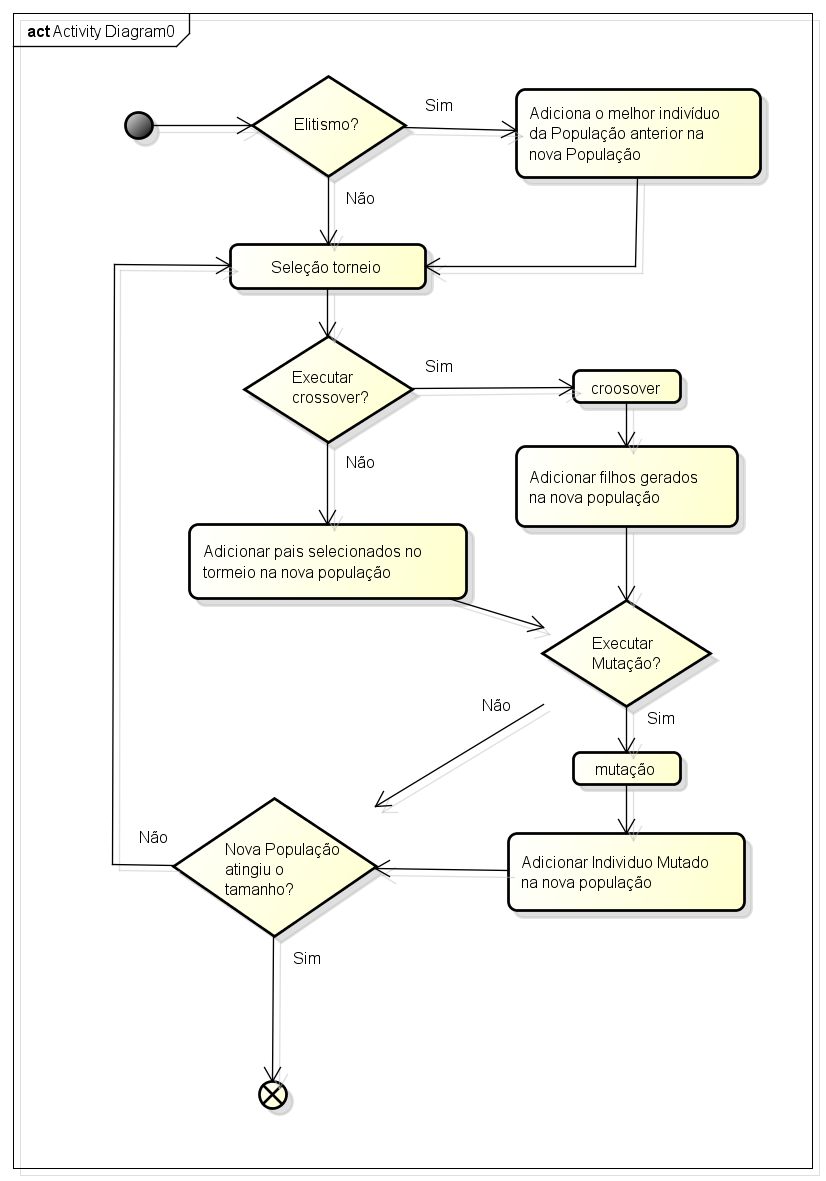
\includegraphics[scale=0.5]{imagens/fluxoNovaPopulacao.png}
\\ \textbf{\footnotesize Fonte: Desenvolvido pelo autor}
\end{figure}

\subsecao{Fluxo do algoritmo}

O fluxo do algoritmo conforme a figura~\ref{fig:fluxoAlgoritmo}, é iniciado pela criação da população inicial. Para cada interação do algoritmo é verificado se a população contém o resultado e se o algoritmo não atingiu o numero de gerações pré-definidas. Se as duas condições forem falsas o algoritmo cria uma nova população.

\begin{figure}[!htb]
\caption[Fluxo do algoritmo]{Fluxo do algoritmo}
\label{fig:fluxoAlgoritmo}
\centering
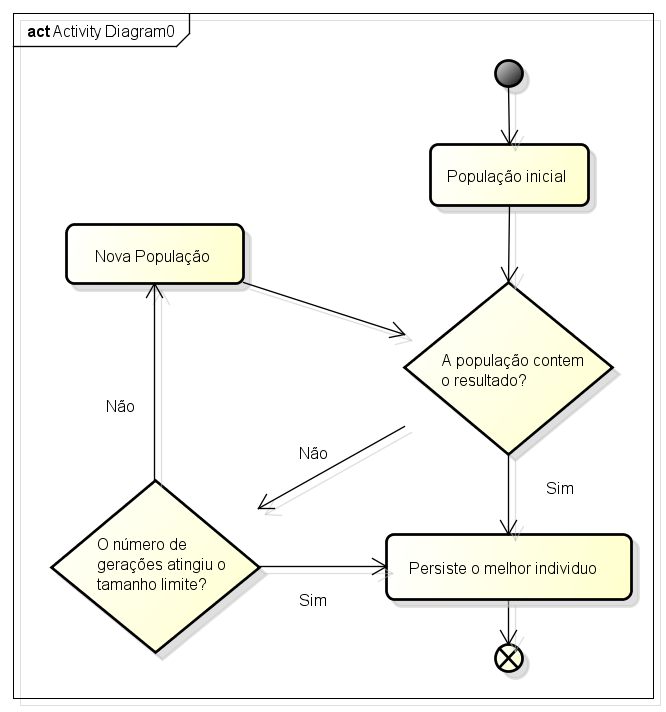
\includegraphics[scale=0.7]{imagens/fluxoAlgoritimo.png}
\\ \textbf{\footnotesize Fonte: Desenvolvido pelo autor}
\end{figure}